
\section{Preliminaries}
\label{section:prelims}
\setcounter{theorem}{0}
\subsection{Notations}
\begin{itemize}
    \item Bit strings $\a$ are in bold, with subscript $a_i$ denoting the $i$-th bit, and $|\a|$ denoting their length. Concatenation is denoted by $||$.
    \item Sans-serif font is for unitaries like $\C$, and the application to a quantum state is $\C[\rho] = \C\rho\C^\dagger$; compositions are written with $\circ$.
    \item Typewriter font is for state labels, like the $\ket\Xlabel = \ket+$ state because $\ket+$ is a $+1$-eigenstate of the Pauli operator $\X$. We also label the magic state for the $\T$-gate as $\ket\Tlabel=\T\ket+$ (see later).
    \item Quantum circuits are sequences of instructions, specified by composition of unitaries like $C=\C_2\circ\C_1$, and end with computational basis measurement of all the qubits.
    \item
    A unitary with an index means that it applies the identity on the unspecified indices. For instance, $\X_n$ is the Pauli $\X$ applied on the $n$-th qubit. An exception in the paper holds for $\C_i$ and $\F_i$, where the index $i$ refers to layers in the circuit, numbered from $1$ to $t$. This will be made explicit later.
    \item For a tensor product $\E$ of $n$ unitaries, let $[\E]_i$ denote the $i$-th unitary of the tensor product ($i\leq n$).
    \item We write the set of angle multiples of $\pi/2$ as $\Theta=\{0, \pi/2, \pi, 3\pi/2\}$.
    \item For a set $S$, writing $s\gets\$ S$ means that $s$ is sampled uniformly at random from $S$.
\end{itemize}

\subsection{Setting}
This work is in the Prepare-and-Send setting, where the Client has the ability to prepare single-qubit states in the set of states $\classA = \{\ket\Tlabel, \pm\ket\Xlabel, \pm\ket\Ylabel, \pm\ket\Zlabel\}$. These are the six single-qubit stabilizer states, and the magic state. The Client is assumed to be perfect. For the Server, three scenarios are examined (see Section~\ref{section:verification}): honest and perfect, honest but noisy, or arbitrarily malicious. In this work we consider quantum computations in the $\BQP$ class (see below), for which the input is a classical bitstring and the output is a decision bit.

\subsection{Quantum Computations}
\label{subsection:prelims:QC}

\paragraph{Bounded-error quantum computation ($\BQP$).}
A language $L$ is in $\BQP$ if there exists a uniform family of polynomial-size quantum circuits $\{C_n\}_{n \in \mathbb{N}}$ and a constant $\bqp < 1/2$ such that for every input $x \in \{0,1\}^n$, the circuit $C_n$ outputs the correct decision bit $z^\star$ for whether $x \in L$ with probability at least $1-\bqp$. This naturally captures general quantum computations with classical inputs and outputs.
Indeed, any $\BQP$ computation resulting in a classical bitstring can be reduced to a polynomial number of decision problems, meaning this definition encompasses the full range of problems solvable by a quantum computer.

In the delegated setting considered in this work, it is more convenient to separate the "input preparation" step from the actual computation machinery. We therefore write $C(\x)$ for a computation that consists of running circuit $C$ on input the input $\ket\x$ provided by the Client. Also, we assume all qubits are measured in the computational basis but only the first one $y=C(\ket\x)$ is kept. Under this convention, correctness requires that
\[
\Pr[y = z^\star] \geq 1-\bqp
\]
for every $\x \in \{0,1\}^n$.

\paragraph{The Pauli and Clifford groups.}
In this work, we write $\mathcal P_n$ for the Pauli group on $n$ qubits, defined as
\[
\mathcal P_n=\{\pm 1,\pm i\}\times \{\id,\X,\Y,\Z\}^{\otimes n}.
\]
By definition, the Clifford group $\mathcal{C}_n$ over $n$-qubits is a subgroup of the unitary group that normalizes the Pauli group: for any $\C\in\Clifford_n$ and any $\P\in\Pauli_n$, we have $\C\P\C^\dagger\in\Pauli_n$. The Clifford group is generated by the single-qubit gates $\H$ and $\P$ (where $\P$ is the $\pi/2$ $\Z$-rotation) together with the two-qubit gate $\CNOT$.

\paragraph{Clifford and $\T$ gates.}
Let $C$ be an $n$-qubit quantum circuit. It is a standard result that the gate set formed by the $n$-qubit Clifford group $\Clifford_n$ and the $\T$-gate, $\T = \mathrm{diag}(1, e^{i\pi/4})$, is universal for quantum computation: any polynomial-size quantum circuit can be efficiently approximated by a circuit composed of these gates \cite{NC00quantum}. Any approximation error arising from this compilation can be absorbed into the overall bounded-error parameter $\bqp$.

Since Clifford gates can permute qubits, we may assume without loss of generality that every $\T$-gate acts on the $n$-th qubit.
In this work, we thus consider the Clifford+T decomposition of any quantum circuit, meaning that for any  $\BQP$ circuit $C$, there exists $t\in\naturals$ such that $C$ can be decomposed as:
\begin{equation}
    C = \C_{t+1} \circ \T_n \circ \C_{t} \circ \cdots \circ \T_n \circ \C_{1},
\end{equation}
where  $\C_i \in \Clifford_n$ are Clifford gates. We refer to the sequence $\{\C_i\}_{i\leq t+1}$ as the \emph{Clifford structure} of the computation, and we say that $C$ is a $(n,t)$-Clifford+$\T$ computation.
This is depicted in Figure~\ref{fig:prelims:C-T}, for $n=3$ and $t=2$ for a readable example. Throughout the paper, we will stick with this example but the results hold for any $n,t$.
\begin{figure}[h]
    \centering
    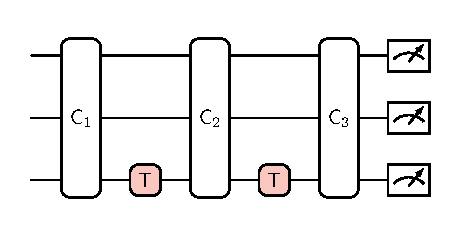
\includegraphics[]{tikz-figures/msi/clifford.pdf}
    \caption{Representation of a $(n=3,t=2)$-Clifford+$\T$ quantum computation.}
    \label{fig:prelims:C-T}
\end{figure}

\paragraph{Measurements.} Without loss of generality, we assume in this paper that measurements are performed in the computational basis. The outcomes are the eigenvalues of the observable $(\id - \Z)/2$, namely $0$ and $1$.

\paragraph{Magic-State Injection \cite{BK04universal}.} In most quantum computing architectures, $\T$-gates are implemented by the use of a Clifford circuit, the injection of an ancillary qubit prepared in a $\T\ket+$ state, a Pauli measurement, and a $\Z$-rotation of angle $\pi/2$ and Pauli $\X$ correction conditioned on the measurement outcome.
Since this specific quantum state allows one to perform the $\T$-gate using Clifford operations only (and a measurement in a Pauli basis, standard in all implementations), it is often referred to in the literature as a \emph{Magic State}. By convention, we write $\ket\Tlabel=\T\ket+$. We also write $\F$ for the circuit consisting of a $\CNOT$ (where the target is the qubit on which the $\T$-gate is intended) followed by a $\SWAP$, as depicted in Figure~\ref{fig:prelims:MSI}.
\begin{figure}[h]
    \centering
    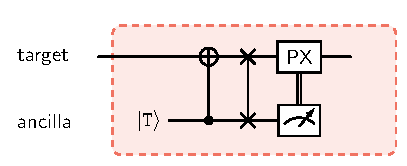
\includegraphics{tikz-figures/msi/msi-single-2.pdf}
    \caption{Magic-State Injection, to implement a $\T$-gate.}
    \label{fig:prelims:MSI}
\end{figure}
In the considered model of computation, the $\T$-gate only acts on the $n$-th qubit, and the $i$-th one uses an ancilla labeled as qubit $n+i$, so we formally define $\F_i=\SWAP_{n+i, n}\circ \CNOT_{n+i, n}$. The circuit of Figure~\ref{fig:prelims:C-T}, on $n$ qubits, becomes the circuit of Figure~\ref{fig:prelims:C-T-MSI}.
\begin{figure}[h]
    \centering
    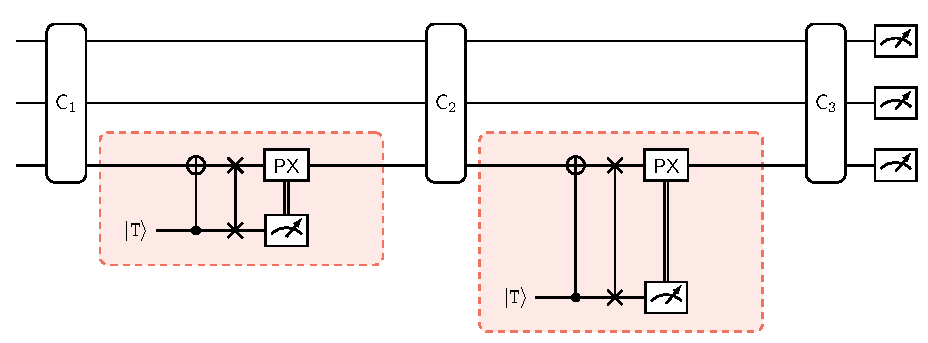
\includegraphics[]{tikz-figures/msi/msi.pdf}
    \caption{
    Representation of a $(3,2)$-Clifford+MSI quantum computation. It is the same as Figure \ref{fig:prelims:MSI} but the $\T$-gates have been implemented \textit{via} Magic-State Injection.}
    \label{fig:prelims:C-T-MSI}
\end{figure}
\paragraph{Stabilizer States.} We say that a state $\ket\psi$ is stabilized by operator $\P$ if $\ket\psi$ is a $+1$ eigenstate of $\P$, meaning $\P\ket\psi=\ket\psi$.
\emph{Stabilizer states} are stabilized by a maximal Abelian subgroup of $\mathcal{P}_n$. For instance, $\ket0$ is stabilized by $\Z$, while $\ket1$ is stabilized by $-\Z$. There are $6$ single-qubit stabilizer states.
By convention, for any $\P\in\Pauli_1$ we will write its $+1$-eigenstate as $\ket {\Plabel}$.

\paragraph{Classical simulation of Quantum Computations.}
By the Gottesman–Knill theorem~\cite{G98heisenberg}, any Clifford circuit $\C\in \Clifford_n$ acting on a $n$-qubit stabilizer input state, followed by Pauli measurements, can be efficiently simulated classically, including the full output distribution.

Furthermore, a Pauli measurement is deterministic if and only if the measured Pauli operator belongs to the stabilizer of the state. In particular, measuring qubit $i$ in the computational basis yields outcome $0$ with certainty iff the output state is stabilized by $\Z_i$, equivalently iff the input state is stabilized by $\C^\dagger \Z_i \C$.
\subsection{Pauli Encryption and Decryption}
\label{prelim:Clifford conjugation}

\paragraph{Bitstring representation of Pauli string up to a phase.}
For any $\P\in\Pauli_n$, we can associate two $n$-bit strings $\a, \r$ such that, up to a global phase: $\P\in \{\pm 1, \pm i\} \times \X^\a\Z^\r$, where $\X^\a = \bigotimes_{i\leq n}\X^{a_i}$.
 Then, the conjugation of $\P$ by a Clifford $\C$ is a mapping from $\a, \r$ to some other bitstrings $\a', \r'$. We write $(\a', \r')=\C(\a, \r)$ the bitstrings such that $\C (\Enc{\a}{\r})\C^\dagger = \Enc{\a'}{\r'}$.

\paragraph{The Quantum One-Time-Pad ($\QOTP$).}
In quantum cryptography, it is common to consider $\a, \r$ as secret keys and encrypt a quantum state $\rho$ by applying the Pauli $\Enc{\a}{\r}$, then decrypt with $\Dec{\a}{\r}$ (or with other keys if the operations between encryption and decryption have changed the keys). This is known as the Quantum One-Time Pad \cite{C05secure}, since from the point of view of a receiver who does not know $\a, \r$, the received state is a probabilistic mixture of the different $\Enc{\a}{\r}[\rho]$ for all the possible values of $\a, \r$. When these keys are sampled uniformly, this yields the following equality:
\begin{equation}
    \sum_{\a, \r\in\{0,1\}^n} \Enc{\a}{\r}[\rho] = \sum_{\P\in\Pauli_n} \P[\rho] = \id_n/2^n.
\end{equation}
This equality is easy to do by hand for $n=1$, then trivial to generalize to the multi-qubit case.

\paragraph{$\QOTP$ via EPR pairs and measurements.}
A $\QOTP$ followed by a quantum communication channel can be replaced by creating an EPR pair, using a quantum channel to send half of it, and applying a Bell measurement. This equivalence is shown using Shor-Preskill's reduction~\cite{SP00simple} with a delayed measurement; see Figure~\ref{fig:QOTP-EPR}.
Throughout the paper, we refer to this replacement as an EPR reduction of the initial protocol.
\begin{figure}[h]
    \centering
    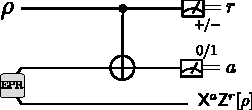
\includegraphics[width=0.5\linewidth]{figures/EPR-OTP.pdf}
    \caption{$\QOTP$ via EPR pairs and measurements. The "EPR" box denotes the creation of an EPR pair, the $+/-$ measurement is in the Hadamard basis, the other is in the computational basis. The outcomes $a, r$ are uniformly distributed.}
    \label{fig:QOTP-EPR}
\end{figure}

\paragraph{Pauli Twirl.}
Applying a random Pauli operator on a quantum state is a recurrent procedure in quantum cryptography or learning since it benefits from the following Twirling lemma.
\begin{lemma}[Pauli Twirl
    ~\cite{DCEL09exact}]
    \label{lemma:Pauli Twirl}
    Let $\rho_n$ be a $n$-qubit quantum state, and let $\E, \E'\in\Pauli_n$. Then:
    \begin{equation}
        \sum_{\Q\in\Pauli_n}
        \Q^\dagger
        \E
        \Q
        \;\rho\;
        \Q^\dagger
        \E^{\prime \dagger}
        \Q
        =0 \; \text{if}\; \E\neq \E'.
    \end{equation}
\end{lemma}
\subsection{Abstract Cryptography Framework}
The Abstract Cryptography (AC) security framework \cite{MR11abstract,M12constructive} used in this work follows the \emph{ideal-world/real-world paradigm}. A protocol is considered secure if it is a good approximation of an \emph{ideal resource} that is secure by design. Its main interest is that protocols that are AC-secure are inherently composable, in the sense that if an AC-secure protocol is used inside a larger protocol, the security of the former does not need to be reproved in the context of the latter. In other words it benefits from sequential and parallel composability.  Ref.~\cite{DFPR14composable} provides an introduction to the topic tailored to verification of quantum computation.

In this framework, the purpose of a secure protocol $\pi$ is, given a number of available resources $\mathcal{R}$, to construct a new resource -- written as $\pi \mathcal{R}$. This new resource can itself be reused in a future protocol. A resource~$\mathcal{R}$ is described as a sequence of CPTP maps with an internal state. It has \emph{input and output interfaces} describing which party may exchange states with it. It works by having each party send it a state (quantum or classical) at one of its input interfaces, applying the specified CPTP map after all input interfaces have been initialized, and then outputting the resulting state at its output interfaces in a specified order. An interface is said to be \emph{filtered} if it is only accessible by a dishonest player. The actions of an honest player $i$ in a given protocol are also represented as a sequence of efficient CPTP maps $\pi_i$ -- called the \emph{converter} of party~$i$ -- acting on their internal and communication registers. We focus here on the two-party Client-Server setting, in which case $\pi = (\pi_C, \pi_S)$. Note that all our protocols are built from quantum channels, due to the Client's requirements to prepare and send single-qubit states.

\paragraph{Indistinguishability of Resources.}

In order to define the security of a protocol, we need to give a pseudo-metric on the space of resources.  We consider for that purpose a special type of converter called a \emph{distinguisher}, whose aim is to discriminate between two resources $\mathcal{R}_1$ and $\mathcal{R}_2$, each having the same number of input and output interfaces.  It chooses the input, interacts with one of the resources according to its own (possibly adaptive) strategy, and guesses which resource it interacted with by outputting a single bit.  The Distinguisher has access to all of the resource's interfaces. Two resources are said to be indistinguishable if no distinguisher can guess correctly with good probability, captured by Definition~\ref{def:ind-res}.

\begin{definition}[Statistical Indistinguishability of Resources]
  \label{def:ind-res}
  Let $\epsilon > 0$, and let $\mathcal{R}_1$ and $\mathcal{R}_2$ be two resources with same input and output interfaces.  The resources are \emph{$\epsilon$-statistically-indistinguishable} if, for all unbounded distinguishers $\mathcal{D}$ the distinguishing probability $p_d$ is bounded by $\epsilon$, meaning if
  \begin{equation}
    \label{eq:dist}
    p_d := \Bigl\lvert\Pr[b = 1 \mid b \leftarrow \mathcal{D}\mathcal{R}_1] - \Pr[b = 1 \mid b \leftarrow \mathcal{D}\mathcal{R}_2]\Bigr\rvert \leq \epsilon.
  \end{equation}
  We then write $\mathcal{R}_1 \underset{\epsilon}{\approx} \mathcal{R}_2$.
\end{definition}

\paragraph{Construction of Resources.}
The construction of a given resource $\mathcal{R}$ by the application of protocol $\pi$ to resource $\mathcal{S}$ can then be expressed as the indistinguishability between resources $\mathcal{R}$ and $\pi \mathcal{S}$.  More specifically, this captures the correctness of the protocol.  The security is captured by the fact that the resources remain indistinguishable if we allow some parties to deviate in the sense that they are no longer forced to use the converters defined in the protocol but can use any other CPTP maps instead.  This is done by removing the converters for those parties in Equation~\ref{eq:dist} while keeping only $\pi_H = \prod_{i \in H} \pi_i$ where $H$ is the set of honest parties.
Since this work only considers an honest-Client / (potentially-)malicious-Server setting, there is only one honest party: the Client, with converter $\pi=\pi_C$, and one potentially malicious party.
The security is formalized as in Definition~\ref{def:ac-sec} in this case, and depicted on Figure~\ref{fig:prelims:AC}.

\begin{definition}[Construction of Resources]\label{def:ac-sec}
    Let $\epsilon > 0$. We say that a two-party protocol $\pi$ $\epsilon$-statistically-constructs resource $\mathcal{R}$ from resource $\mathcal{S}$ if:
    \begin{enumerate}
        \item It is correct: $\pi \mathcal{S} \underset{\epsilon}{\approx} \mathcal{R}\filter$, where $\filter$ prevents malicious behavior (from the potentially cheating party);
        \item It is secure against malicious party $P$: there exists a \emph{simulator} (converter) $\sigma$ such that $\pi\mathcal{S} \underset{\epsilon}{\approx} \mathcal{R} \sigma$.
        \label{item:prelim:AC-security}
    \end{enumerate}
\end{definition}

\begin{figure}[h]
    \centering
    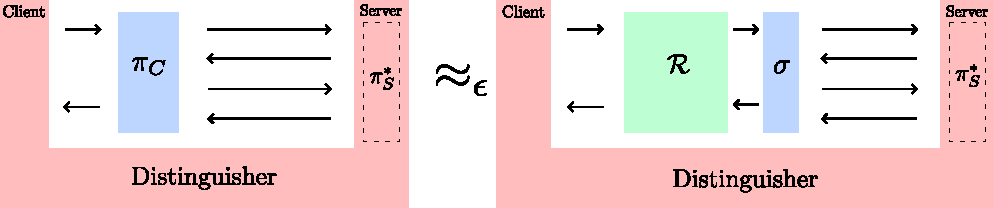
\includegraphics[width=\linewidth]{figures/prelims-AC.pdf}
    \caption{Security in Abstract Cryptography: indistinguishability between the Real World (left picture) and the Ideal World (right picture) up to distance $\epsilon$.
    In each scenario, the Distinguisher (red box) has two interfaces: Client and Server.
    Its inputs are fixed in both scenarios: the Distinguisher chooses the protocol's inputs from the Client interface, and chooses an arbitrary malicious behavior from the Server interface, captured by a CPTP map $\pi_S^*$, that respects the interface of the Client protocol $\pi_C$.
    The protocol is $\epsilon$-secure if the Distinguisher guesses correctly with probability at most $\epsilon$ if it was interacting with the Client Protocol $\pi_C$ (blue box, left picture) in the Real World or the Simulator $\sigma$ (blue box, right picture) plugged in the Resource $\mathcal R$ in the Ideal World.
    }
    \label{fig:prelims:AC}
\end{figure}

\paragraph{Composition of Resources.}
Using the definitions above, we can state the following general composition theorem~\cite{MR11abstract} that guarantees the additive accumulation of distinguishing advantage when composing two statistically secure protocols.
\begin{theorem}[General Composition of Resources~\cite{MR11abstract}]
  Let $\mathcal{R}$, $\mathcal{S}$ and $\mathcal{T}$ be resources, $\alpha, \beta$ and $\mathsf{id}$ be protocols, where protocol $\mathsf{id}$ does not modify the resource it is applied to.  Let $\circ$ and $|$ denote the sequential and parallel composition of protocols and resources, respectively.  Then the following implications hold:
  \begin{itemize}
  \item Sequential composability: if $\alpha \mathcal{R} \approx_{\epsilon_{\alpha}} \mathcal{S}$ and $\beta\mathcal{S} \approx_{\epsilon_{\beta}} \mathcal{T}$, then $\left(\beta \circ\alpha\right) \mathcal{R} \approx_{\epsilon_{\alpha}+\epsilon_{\beta}}\mathcal{T}$.
  \item Parallel composability (context insensitivity): if $\alpha \mathcal{R} \approx_{\epsilon_{\alpha}} \mathcal{S}$, then $\left(\alpha \mid \mathrm{id}\right)\left(\mathcal{R} \mid \mathcal{T}\right) \approx_{\epsilon_{\alpha}} \left(\mathcal{S} \mid \mathcal{T}\right)$.
  \end{itemize}
  Combining these two properties yields the composability of protocols.
\end{theorem}

